\documentclass{standalone}
\usepackage[utf8]{inputenc}
\usepackage{newtxtext}
\usepackage{newtxmath}
\usepackage[italic]{hepnicenames}
\makeatletter\def\@shiftlen@anti@gen@bar{0mu}\makeatother
\usepackage[svgnames]{xcolor}
\usepackage{tikz-feynhand}


\begin{document}
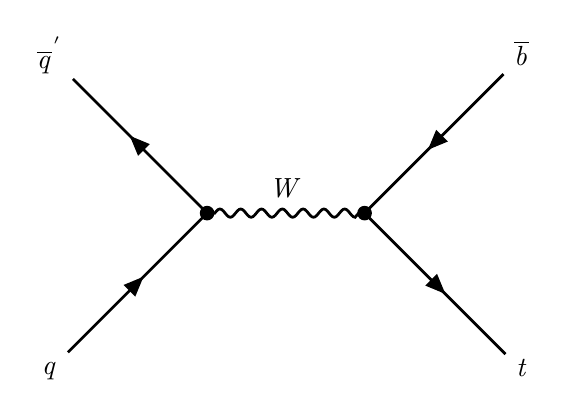
\begin{tikzpicture}
  \setlength{\feynhandlinesize}{1.0pt}
  \tikzfeynhandset{every dot={/tikz/color=Black},}
  \begin{feynhand}
    \vertex [particle, Black] (q1) at (-3.0, 2.0) {$\Paq^{'}$};
    \vertex [particle, Black] (q2) at (-3.0, -2.0) {\Pq};
    \vertex [particle, Black] (b) at (3.0, 2.0) {\Paqb};
    \vertex [particle, Black] (t) at (3.0, -2.0) {\Pqt};
    
    \vertex [dot, Black] (qq) at (-1.0, 0.0) {};
    \vertex [dot, Black] (bt) at (1.0, 0.0) {};
    
    \propagator [fermion, Black] (qq) to (q1);
    \propagator [fermion, Black] (q2) to (qq);
    \propagator [boson, Black] (qq) to [edge label=\PW, color=Black] (bt);
    \propagator [fermion, Black] (b) to (bt);
    \propagator [fermion, Black] (bt) to (t);
  \end{feynhand}
\end{tikzpicture}
\end{document}
